\chapter{Cooling}
\label{chap:Cooling}
A prerequisite for performing photon recoil spectroscopy, is that the system which is investigated, is cooled to the quantum mechanical ground state of its motion.
Cooling of ions in linear Paul traps usually occurs in two stages. First the ion(s) is cooled to approx. 1mK by Doppler cooling, as is described in \cref{sec:Doppler}.

When the ion(s) has been cooled to mK tempearture by Doppler cooling, it starts exhibiting quantum mechanical properties. Since the potential in the trap is harmonic, the wavefunction of the ion(s), is that of the harmonic oscillator.
To reach the quantum ground state, it is necessary to perorm sideband cooling which takes the ion(s) from whichever $\vert n\rangle$ state it starts in, and moves it to the state $\vert0\rangle$ of the harmonic oscillator. This process is described in \cref{sec:SBC}.

Finally there may be some complications to the above cooling processes if we consider two ions with very large charge-to-mass mismatch as explained in \cref{sec:2Ion}. \Cref{sec:Coupling}
\section{Doppler cooling}
\label{sec:Doppler}
The very first part of cooling two ions down consists of Doppler cooling \textcolor{red}{WINELAND}. This method of laser cooling was pioneered by David Wineland and relies on detuning laserlight with respect to an internal transition of the ion, in order to effectively generate a drag force on the ion, cooling it down.

An ion in motion experiences, with a velocity $\vec{v}$, experiences a Doppler shift of laser light with wave vector $\vec{k}$ according to
\begin{equation}
    \omega_{obs} \approx (1-\vec{k}\cdot\vec{v})\omega_L,
\end{equation}
where $\omega_{obs}$ is the frequency seen by the ion, and $\omega_L$ is the frequency of the laser in the laboratory frame.
Thus if we detune the light of the laser to be below the frequency of an electronic transition in the ion $\omega$, the ion will preferentially absorb photons, when it is propagating against the direction of the light.
Due to conservation of momentum, the ion must change its momentum by
\begin{equation}
    \Delta\vec{p} = \hbar\vec{k}.
\end{equation}
After a short time the ion will decay to the ground state once again, but since the direction of the photon emitted during decay is symmetric, this will, if averaged over multiple emissions, lead to no change in momentum.
Thus the momentum of the ion is effectively decreased, since the ion preferentially absorbs photons propagating in the oppsite direction of itself. At low velocities $kv\ll\Gamma$, where $\Gamma$ is the decay rate of the excited state, one can express this as a drag force (assuming 1D problem to ease notation) \textcolor{red}{KARIN}:
\begin{equation}
    F_{drag} = -\beta v,\quad \beta = \frac{8\hbar s k^2\delta / 2\Gamma}{\big(1+s+(2\delta/\Gamma)^2\big)^2},
\end{equation}
where $\beta$ is the drag coefficient, $\delta = \omega_L-\omega$ is the detuning of the laser with respect to the atomic transition, $s = I/I_{sat}$ is the saturation parameter, where $I$ is the intensity of the laser light, and $I_{sat} = \frac{\pi hc}{3\lambda}\Gamma$, with $\lambda$ being the wavelength of the laser, is the saturation intensity of the transition. 

It is important to note, that while the equation above seems to indicate that there is no limit to Doppler cooling, that is far from the case. Indeed since the direction of an emitted photon is random, the ion will perform a random walk in momentum space over time.
Thus, there is an intrinsic variation of velocity over time, meaning there is a lower limit to the temperature of the ion (typically referred to as the Doppler temperature or Doppler limit), which is given by
\begin{equation}
    T_D = \frac{\hbar\Gamma}{2k_b}\label{eq:DopplerTemp},
\end{equation}
which for the case of Ba$^+$ this temperature is approx. 0.5mK.

Of course Doppler cooling only works for very specific ions, that have the proper level-scheme, and is thus not a very good candidate for cooling arbitrary molecular ions.
The solution to this problem of not being able to doppler cool molecular ions comes in two parts. Firstly at high temperatures the hot molecular ion will interact with the cooled atomic ions, via the Coulomb interaction. Such interactions will cause the molecular ion to transfer energy to the atomic ion, from which the energy will then be removed by the system via Doppler cooling. This method of cooling is called sympathetic cooling \textcolor{red}{CITE MICHAEL (2000) AND REVIEW by Willitsch}
In this case we imagine ideally trapping the molecule with a large amount of Ba$^+$ ions to offer the most cooling.

As temperatures drop low enough that the motion truly becomes harmonic, the motion of the ions becomes coupled. As such, the ions will have common motional modes, and any energy extracted from the Ba$^+$ ion is extracted from the mode as a whole, thus cooling the molecular ion as well.
This cooling mechanism is only effective if the ions share similar mass-to-charge ratios, however. In the case where the ion motions are nigh uncoupled, as described in \cref{sec:2Ion}, further steps must be taken to get the molecular ion to mK temperatures. This is described in \cref{sec:Coupling}.


\section{Sideband Cooling}
\label{sec:SBC}
Unfortunately, Doppler cooling is not sufficient for reaching the motional ground state. In order to do this we employ yet another method of laser cooling, called sideband cooling \textcolor{red}{cite}. When the ions are at the doppler temperature, they will be cold enough that they behave as a quantum mechanical harmonic oscillator, with their wave function
being a thermal distribution over the Fock states $\vert n \rangle$. By coupling the state $\vert g,n\rangle$ to the state $\vert e,n-1\rangle$ where $(e,g)$ denotes the excited and ground states of the atom, we are able to remove one quanta of energy from the motion under an excitation of the electronic state.
Since the electronic state predominantly decays to the same $n$, this allows us to cool the ion's motion by moving down the "ladder" seen on \cref{fig:SBC}


We initially consider a single atomic ion in the Paul trap, and neglect the radial modes of motion in order to ease notation. The Hamiltonian can be written as
\begin{equation}
    \hat{H}_0 = \hbar\omega_{z}(\hat{n}+1/2)+\hat{H}_a,
\end{equation}
where $\hat{n}$ is the Fock state number operator, and $\hat{H}_a$ is the Hamiltonian for the atomic system. If a laser field is turned on at some detuning $\delta = \omega_L -\omega$ with respect to the electronic transition of the ion, the interaction with the laser in the interaction picture is described by:
\begin{equation}
    H_{I} = \frac{\hbar\Omega_0}{2}\hat{\sigma}_+\big(e^{ik_z\hat{z_I}}e^{-i\delta t}\big) + h.c.,
    \label{eq:interaction}
\end{equation}
where $\hat{\sigma}_+ = \vert e \rangle \langle g \vert$ is the excitation operator responsible for exciting the electronic state of the ion, and $\Omega_0 = \frac{eE_0}{\hbar}\langle g \vert \hat{\epsilon}\cdot\hat{z}\vert e\rangle$ is the Rabi frequency of the transition, being driven by an electric field of amplitude $E_0$, and direction $\hat{\epsilon}$. Note that the rotating wave approximation has been applied to the expression above, keeping only slowly rotating terms.

We may express $\hat{z}_I$ in terms of the ladder operators yielding
\begin{equation}
    \hat{z}_I = \sqrt{\frac{\hbar}{2m\omega_z}}(\hat{a}e^{-i\omega_z t}+\hat{a}^\dagger e^{i\omega_z t})
\end{equation}
Before inserting this expression back into \cref{eq:interaction}, it will be useful to first define the Lamb-Dicke parameter
\begin{equation}
    \eta = k_z\sqrt{\frac{\hbar}{2m\omega_z}},
\end{equation}
which in the so-called Lamb-Dicke regime, where $\eta\sqrt{\langle n \rangle +1} \ll 1$ \textcolor{red}{EMILIE} allows us to write
\begin{equation}
    H_I = \frac{\hbar\Omega_0}{2}\hat{\sigma}_+\bigg[e^{-i\delta t} + i\eta\big(\hat{a}^\dagger e^{i(\omega_z -\delta)t}+\hat{a}e^{-i(\omega_z+\delta)t}\big)\bigg] + h.c.
\end{equation}
Here the first term is resonant when $\delta = 0$ and corresponds to the laser being resonant with the atomic transition, driving it with no change in motional quantum number. The second term is resonant when the laser is blue detuned by  $\delta = \omega_z$, and increases the motional quantum number while exciting the system, thus heating the system, corresponding to walking up the ladder of \cref{fig:SBC}.
Finally the third term is resonant when $\delta = -\omega_z$, and removes a phonon at by performing an electronic excitation. Repeatedly performing this process will eventually cool the ion to the ground state, as seen on \cref{fig:SBC}.

If we instead consider two ions, the picture changes ever so slightly. In the case where only one of the ions interacts with the laser light, as would be the case for Ba$^+$ cotrapped with a molecule, we simply have to include the mode structure when writing out $\hat{z}_1$. In the case of two ions with in-phase and out-of-phase frequencies of $\omega_i,\omega_o$, the motional state of the system is described by the product space $\vert n_i,n_o\rangle$.
Where the subscript ($i/o$) denotes the in-phase and out-of-phase mode respectively. The position operator for the barium ion in this system can be expressed as

\begin{equation}
    \hat{z}_1 = \sqrt{\frac{\hbar}{2m_1}}\bigg(\alpha_{i,1}\frac{a_i+a_i^\dagger}{\sqrt{\omega_i}}+\alpha_{o,1}\frac{a_o+a_o^\dagger}{\sqrt{\omega_o}}\bigg),
\end{equation}
where $\alpha_{i/o,1}$ is the participation of the atomic ion in the motion of the mode, as calculated in \cref{sec:2Ion}. This operator may be inserted in the place of $z_I$ (remembering to switch to the interaction picture) in equation \cref{eq:interaction}. Following an identical derivation we see that sideband cooling is still possible for all modes, provided that $\alpha_{i/o}$ does not get so small, that the coupling becomes too weak.

This clearly poses a problem for systems where the mass-to-charge ratios of the two ions differ considerably, as $\alpha_{i,1}\ll \frac{1}{\sqrt{2}}$ for such systems. Effectively making cooling of the in-phase motion impossible.

\begin{figure}
    \centering
    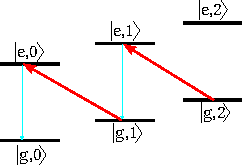
\includegraphics[width = 0.8\textwidth]{main/coolingScheme.pdf}
    \caption{Illustration of the concept behind sideband laser cooling. The laser (red) is detuned with respect to the electronic transition, by exactly $\omega_z$. Thus transitions are driven at the cost of a phonon. The atom is most likely to decay to the same Fock state, effectively causing it to lose phonons, as several excitations occur. This makes the ion "climb down the ladder" until it reaches the quantum ground state.}
    \label{fig:SBC}
\end{figure}

\section{Coupling of motional modes to enhance cooling}
\label{sec:Coupling}
As mentioned in both \cref{sec:Doppler} and \cref{sec:SBC}, laser cooling becomes very difficult once the charge-to-mass ratios of the two differ considerably. The reason for this is relatively easy to understand.
Since the laser cooling only interacts with the atomic ion, this is the only ion whose motion is cooled through the interaction with the light. In the case where the ions have similar charge-to-mass ratios however, their motions are so strongly coupled, that any cooling of the atomic ion, will cool the molecular ion as well.
As the ratios start to differ the motions quickly become uncoupled, and thus the cooling of the atom, no longer affects the molecule in any appreciative way. This is clearly seen on \cref{fig:WCMSCM}, which shows the temperature of Ba$^+$ ion, cotrapped with a polyporphyrine ($m_2 = 9000$ amu, $q_2 = 24$e). The blue curve shows the temperature of the motional modes, that have a large contribution from the atom. Clearly these modes are effectively cooled. In stark contrast we have the orange curve, which displays the temperature of all the modes that have low contribution from the atom, whose temperature remains effectively unchanged.

\begin{figure}
    \centering
    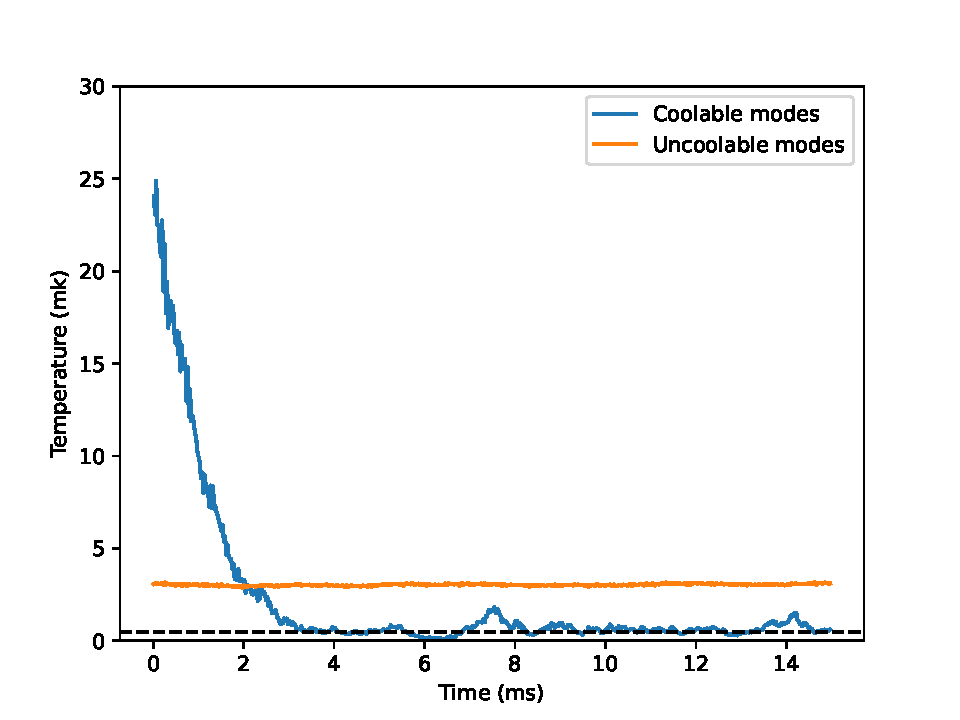
\includegraphics[width = \textwidth]{main/WCM_SCM_Temp.pdf}
    \caption{Simulation of Doppler cooling of a two/ion system, containing of a Ba$^+$ ion, and a polyporphyrin. Two curves are plotted, corresponding to the tempearture of the modes with high (blue), and low (orange) participation from the Ba$^+$ ion. Clearly only the modes with a high participation are cooled by the Doppler cooling}
    \label{fig:WCMSCM}
\end{figure}

In fact, this problem reaches further than simply cooling. For example, it is the molecular ion we wish to investigate with photon recoil spectroscopy (PRS). However the momentum kick gained from absorption on the molecule, will predominantly excite the motional modes with high participation from the molecule.
Unfortunately the readout method for PRS is very similar to the side-band pulses described in \cref{sec:SBC}, and thus for the same reasons, readout becomes impossible when the coupling grows too weak, since these modes have very small participation from the atomic ion, on which readout is performed.


The solution to this problem is to find some way to couple the two modes, allowing for the transfer energy from one to the other. Curiously enough the need for coupling such modes was present in Penning traps many years ago, in order to cool the so-called magnetron mode of such a trap \cite{PenningTrap,DehmeltPenningCool}. For the Pennin trap the solution found was to add another quadrupole field, oscillating at the frequency difference between the two modes to be coupled, such a solution also works for the case of the Paul trap as has been demonstrated very recently \textcolor{red}{CITE REFEREE}.

It is easiest to understand the coupling that occurs, when we consider the quantum mechanical case. Suppose we introduce some additional potential (by modulating a slight additional voltage on the endcap electrodes)
\begin{equation}
    V'(z_1,z_2,t) = \frac{\kappa V_0}{z_0^2}(q_1z_1^2+q_2z_2^2)\cos{\big([\omega_i-\omega_o]t\big)}\label{eq:couplingPot},
\end{equation}
where $V_0$ is the additional voltage put onto the endcap electrodes. We note that $V_0$ is kept small with respect to $V_{DC}$, such that the eigenmodes of the system are not considerably changed.

If we perform a Taylor expansion to second order around the equilibrium (at $V_0= 0$) positions is performed similarly to \cref{sec:2Ion}, we may write (neglecting the offest term)
\begin{align}
    V'(\delta z_1,\delta z_2,t)\approx &\frac{\partial V'}{\partial z_1}\bigg\vert_{eq}\delta z_1+\frac{\partial V'}{\partial z_2}\bigg\vert_{eq}\delta z_2
    +\frac{1}{2}\frac{\partial^2 V'}{\partial z_1^2}\bigg\vert_{eq}\delta z_1^2\nonumber\\+&\frac{1}{2}\frac{\partial^2 V'}{\partial z_2^2}\bigg\vert_{eq}\delta z_2^2
    +\frac{\partial^2 V'}{\partial z_1\partial z_2}\bigg\vert_{eq}\delta z_1\delta z_2.
\end{align}
For now, we only wish to consider the coupling of the modes, and thus neglect the first-order terms. Clearly these terms cannot couple the modes as $\delta\hat{z}_j\propto (\alpha_{j,o}\hat{a}_o+\alpha_{j,i}\hat{a}_i)+h.c.$ is not sufficient to transfer energy from one mode to another. If we instead consider solely the 2nd. order terms we find
\begin{align}
    \hat{V}'^{(2)} = \nonumber \frac{\hbar\kappa V_0}{2z_0^2}\cos{\big([\omega_i-\omega_o]t\big)}\bigg(&q_1\big(\frac{\alpha_{1,i}(\hat{a}_i+\hat{a}_i^\dagger)}{\sqrt{m_1\omega_i}}+\frac{\alpha_{1,o}(\hat{a}_o+\hat{a}_o^\dagger)}{\sqrt{m_1\omega_o}}\big)^2\\
    &+q_2\big(\frac{\alpha_{2,i}(\hat{a}_i+\hat{a}_i^\dagger)}{\sqrt{m_2\omega_i}}+\frac{\alpha_{2,o}(\hat{a}_o+\hat{a}_o^\dagger)}{\sqrt{m_2\omega_o}}\big)^2\bigg).
\end{align}
If the cosine is expanded using Euler's formula, and we move to the interaction picture, keeping only the non-rotating terms, we may massage the expression and eventually arrive at
\begin{equation}
    \hat{V}'^{(2)}_I = \frac{\hbar\kappa V_0\alpha_{1,o}\alpha_{1,i}}{4z_0^2\sqrt{\omega_i\omega_o}}\big(\frac{q_1}{m_1}-\frac{q_2}{m_2}\big)(\hat{a}_o^\dagger \hat{a}_i + h.c.),
\end{equation}
for which it is clear that the two modes of motion are coupled. We define $g_0 = \frac{\kappa V_0\alpha_{1,i}\alpha_{1,o}}{4z_0^2\sqrt{\omega_i\omega_o}}(\frac{q_1}{m_1}-\frac{q_2}{m_2})$, that we may write the coupling potential as 
\begin{equation}
    \hat{V}_I'^{(2)} = \hbar g_0(\hat{a}_i^\dagger \hat{a}_o + h.c.).
\end{equation}
It can be shown, that in the coupled system the time-dependent operators $\hat{a}_{i/o}^\dagger(t)$, are given by \cite{hou2022coherently}
\begin{align}
    &\hat{a_i}^\dagger(t) = \hat{a}_i^\dagger(0)\cos(g_0t) + i\hat{a}_o^\dagger\sin(g_0t),\\
    &\hat{a_o}^\dagger(t) = \hat{a}_o^\dagger(0)\cos(g_0t) + i\hat{a}_i^\dagger\sin(g_0t).
\end{align}
For which it is particularly interesting to note that for times $\tau_n = \frac{(2n+1)\pi}{2g_0}$, where $n$ is an integer, we find that $\hat{a}_i^\dagger(\tau_n) = \hat{a}_o^\dagger(0)$, and similarly for $\hat{a}_o^\dagger(\tau_n)$. In addition, we may write any arbitrary state of the system as
\begin{equation}
    \vert \Psi(t)\rangle = \sum_{m,n = 0}^\infty \frac{c_{mn}}{\sqrt{m!n!}}\big(a_i^\dagger(t)\big)^m\big(a_o^\dagger(t)\big)^n\vert 0\rangle_i\vert 0\rangle_o,
\end{equation}
where the values $c_{mn}$ are determined by the initial state of the system, and $\sum c_{mn} =1$.
The action of the coupling is thus clear. In general the cause the two states to oscillate in and out of entanglement, and specifically for times $t = \tau_n$ the states for the two modes become swapped.
This is very beneficial for cooling, since we may cool the mode with high participation from the Ba$^+$ ion, perform a swap, and then cool again. This procedure should, in principle, lead to both modes being in their ground states.


The mode coupling also exists in the classical regime. \Cref{fig:polyPorCooling} shows a simulation of Doppler cooling of a system consisting of a  Ba$^+$ ion, and a polyporphyrin, while the coupling $V'$ is turned on. The results from this simulation stand in stark contrast to those of \cref{fig:WCMSCM}, where the temperature of the molecule is largely unchanged.
\begin{figure}[h]
    \centering
    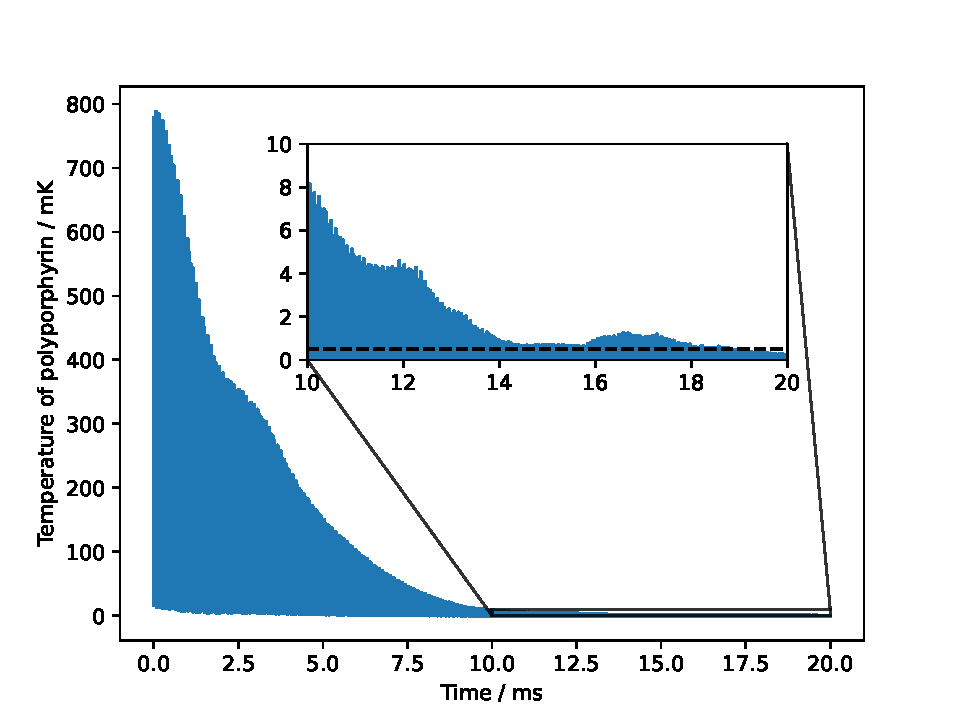
\includegraphics[width = 0.8\textwidth]{main/PolyPorCooling.pdf}
    \caption{Simulation results for Doppler cooling of a system consisting of Ba$^+$ ion and polyporphyrin, while the coupling potential from \cref{eq:couplingPot} is turned on. Unlike the case with no coupling \cref{fig:WCMSCM}, the molecule is cooled efficiently.
    The inset shows temperatures in the span $ t = $10ms to $t = $20ms, as temperatures grow so small that they are not clearly seen on the full figure. The black dotted line shows $T = 0.5$mK, which is the Doppler temperature, calculated by \cref{eq:DopplerTemp}.}
    \label{fig:polyPorCooling}
\end{figure}

In the derivations of this chapter we have ignored the 1st order terms of the Taylor expansion of the potential. In reality, these terms will play a role in the dynamics of the system, since they drive the ions at a frequency, which is similar to their motional frequencies. There are several ways to combat these first order driving terms.
One option, which has been implemented for the case of segmented microtraps, is engineering the field curvature in order to ensure the first order derivatives go to zero at the equilibrium locations of the ions \cite{WeaklyCoupled}. 

Since our trap has considerably fewer segments, such an approach is expected to be difficult to realize in our setup.
The second approach accepts that the driving terms will lead to heating, but attempts to move this heating into the modes, which are easily cooled, i.e. the ones with high participation from Ba$^+$. This can be done by biasing voltages slightly, such that the transfer potential $V'(z_1,,z_2,t)$ has its minimum at $z_{2,eq}$, instead of $z=0$.
We believe this would be relatively simple to implement in the current trap, as a similar thing is already done in order to compensate for micromotion.



The usefulness of this mode-coupling doesn't stop at laser cooling. As mentioned previously when performing PRS, we will largely excite the motion of the molecule, due to the absorption of light via the molecule. Mode-coupling allows for the efficient mapping of the motion of the molecule onto the motion of the ion, resulting in much higher measurement efficiency, and speed.


In addition to the contents of this report, the contents of \cref{chap:LinTrap} and the current chapter have also been used in the authoring of a paper, proposing an experiment to set bounds on a quantum collapse model, known as the continuous spontaneous localization model \cite{lenlereriksen2023testing}. Using the theory of \cref{sec:2Ion}, we found the strongest bounds on the models parameters could be set by performing measurements on the modes with high participation from the molecular ion, yielding another case where mode-coupling can be highly beneficial.
